\documentclass[../TinyBot.tex]{subfiles}
\begin{document}

\section{Intro To Programming Arduinos}

To program an Arduino, you will need a USB cable, and a laptop/computer with the \href{https://www.arduino.cc/en/software}{Arduino IDE} installed. 



\begin{figure}[h]
    \centering
    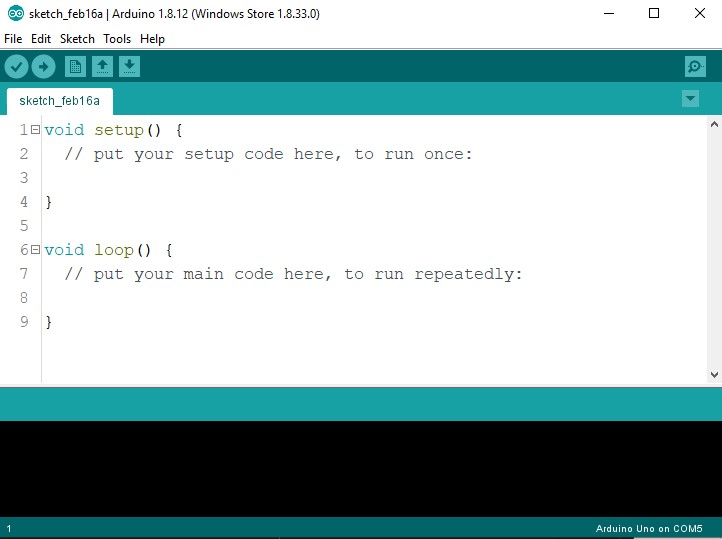
\includegraphics[width=0.7\textwidth]{arduino_ide.jpg}
    \caption{The Arduino IDE}
\end{figure}

The two round buttons in the top right, the tick and the arrow, are the verify and upload buttons. Verify checks your code, making sure that the syntax (the structure of the code, think of it like a grammar checker) of your code is correct. Upload sends the code you've written to the Arduino board.  \\

However, before you can upload your code there's some setup you need to do. First of all, you need to select the board by going into the Tools menu, as shown in the image below. 

\begin{center}
  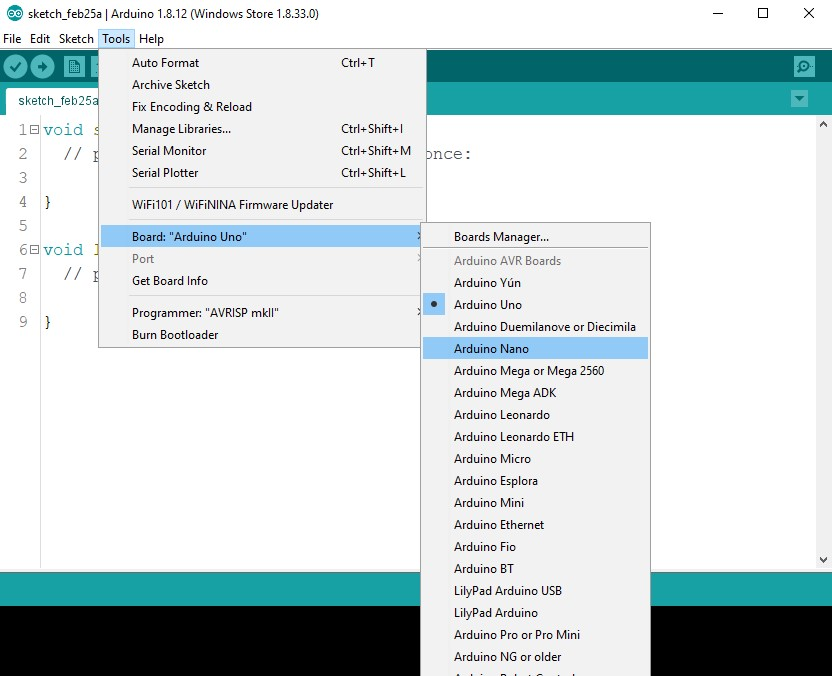
\includegraphics[width=0.6\textwidth]{arduino_ide_select_board.jpg}
  \captionof{figure}{Selecting Board}
\end{center}

Next, you need to select the USB port that the Arduino is connected to. This is also done through the Tools menu. 
\begin{center}
  
\end{center}

The next few paragraphs will explain what programming is, if you have programmed before feel free to skip past these paragraphs. 

Arduino's are programmed in the programming language \lstinline[]!C++!; though there are a few differences. The below code section details a few features of coding.


\begin{lstlisting}
// this is a comment

// variables declared not in a function will be accessible
// in all functions
int global_var = 0;

void setup {
  // everything in this function will run once
  // this code will run when the board is powered on, 
  // or when the reset button is pressed
}

void loop {
  // everything in this function will run repeatedly
}

\end{lstlisting}
\bigskip

\pagebreak
A useful feature of the Arduino IDE is all the example code which is provided.
\begin{center}
    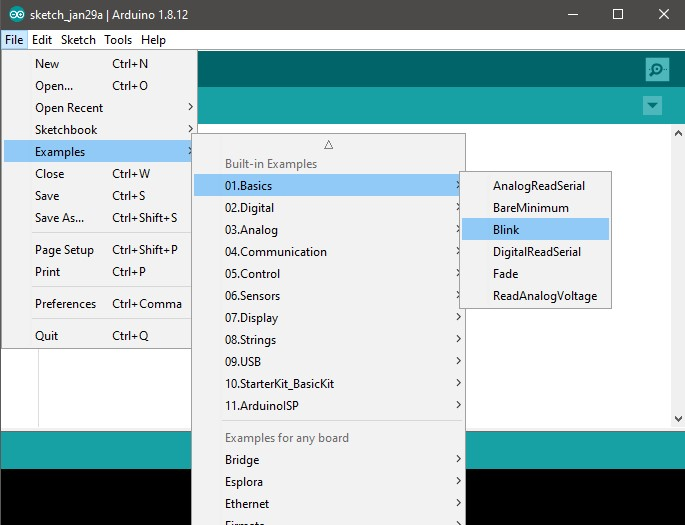
\includegraphics[width=0.7\textwidth]{arduino_ide_blink_example.jpg}
    \label{fig:ide-blink}
    \captionof{figure}{Arduino IDE Example Code}
\end{center}

The simplest Arduino example is the Blink code, which turns on and off an onboard LED.

\begin{lstlisting}
void setup() {
  // initialize digital pin LED_BUILTIN as an output.
  pinMode(LED_BUILTIN, OUTPUT);
}

// the loop function runs over and over again forever
void loop() {
  // turn the LED on (HIGH is the voltage level)
  digitalWrite(LED_BUILTIN, HIGH); 

  delay(1000);      // wait for a second

  // turn the LED off by making the voltage LOW
  digitalWrite(LED_BUILTIN, LOW);  
  
  delay(1000);      // wait for a second
}
\end{lstlisting}


There are a few common aspects present in the code of nearly every Arduino project, no matter how simple or complicated. \\


\lstinline[]!pinMode(<pin number>, <mode>)! sets a digital pin on the Arduino to be either an \lstinline[]!INPUT! or and \lstinline[]!OUTPUT!. \\


\lstinline[]!digitalWrite()! is used to set digital pins \lstinline[]!HIGH! and \lstinline[]!LOW!.

\end{document}